
\documentclass[11pt,a4paper,twoside]{article}
\usepackage[utf8]{inputenc} % Enables direct typing of special characters
\usepackage{url}
\usepackage{todonotes}
\usepackage{tabularx}

% Report title
\newcommand{\theShortTitle}{Recognising Accents using Machine Learning} 

% Recognising Accents using Machine Learning

% Group
\newcommand{\theTitle}{{\Large Intro to AI Group 27} \\ \theShortTitle}

% Group Members
\newcommand{\theAuthors}{Finn McFall, Callum Paton, Leo Pitsillides, Chris Sharp}
\title{\theTitle}
\author{\theAuthors}
\date{\today}

\usepackage[a4paper,top=2.5cm,bottom=2.5cm,left=2.75cm,right=2.75cm,marginparwidth=2.25cm,includeheadfoot,twoside]{geometry}
\usepackage{fancyhdr}
\pagestyle{fancy}
\headheight=18pt
\footskip=18pt
\fancyhf{}

\fancyhead[L]{\bfseries \theShortTitle}
\fancyhead[R]{\bfseries \thepage}
\renewcommand{\headrulewidth}{1pt} 
\usepackage[style=numeric]{biblatex} %Imports biblatex package
\addbibresource{references} %Import the bibliography file
\usepackage{csquotes}
% Line spacing
\usepackage[skip=0.8\baselineskip,indent=0pt]{parskip}

% AMS Packages for maths typesetting
% NOTE: These are extremely useful!!!
\usepackage{amsmath}
\usepackage{amsfonts}
\usepackage{amssymb}

\usepackage{graphicx}
\graphicspath{{./}{./Figures/}}
\usepackage{float}
\usepackage{tikz}
\usepackage{pgfplots}
\pgfplotsset{compat=1.15}
\usetikzlibrary{calc}
\usetikzlibrary{plotmarks}
\usetikzlibrary{patterns}
\usetikzlibrary{shapes}
\usetikzlibrary{positioning}
\usepackage{listings}

\usepackage[english]{babel}       % Hyphenation etc. for English words
\usepackage{color}                % Colours for text
\definecolor{mygreen}{RGB}{28,172,0} % color values Red, Green, Blue
\definecolor{mylilas}{RGB}{170,55,241}
\usepackage{lipsum}               % Filler text "Lorem ipsum dolor sit amet..."
\usepackage{hhline}               % Better lines in tables
\usepackage{todonotes}
\newcommand{\de}{\mathrm{d}}
\newcommand{\diff}[2]{\frac{\mathrm{d} #1}{\mathrm{d} #2}}
\newcommand{\ddiff}[2]{\frac{\mathrm{d}^2 #1}{\mathrm{d} #2^2}}
\newcommand{\pdiff}[2]{\frac{\partial #1}{\partial #2}}

% In text
\newcommand{\ie}{\emph{i.e.}}
\newcommand{\eg}{\emph{e.g.}}
\newcommand{\etc}{\emph{etc.}}

% Useful functions
\newcommand{\floor}[1]{\left\lfloor #1 \right\rfloor}
\newcommand{\ceil}[1]{\left\lceil #1 \right\rceil}

% Extra operator names
% NB. This means that 
\newcommand{\erf}{\operatorname{erf}}
\newcommand{\sech}{\operatorname{sech}}
\newcommand{\csch}{\operatorname{csch}}
\newcommand{\signum}{\operatorname{\text{sgn}}}

% Hyperlinking within text.
% NOTE: This must always be the last part of the preamble (before the doucment)
\usepackage{hyperref}
\hypersetup{
	unicode=true,                 % non-Latin characters in Acrobat bookmarks
	pdftoolbar=true,              % show Acrobat toolbar?
	pdfmenubar=true,              % show Acrobat menu?
	pdffitwindow=true,            % page fit to window when opened
	pdftitle={\theShortTitle},    % title of pdf document
	pdfauthor={\theAuthors},      % author of pdf document
	pdfsubject={},                % subject of the document
	pdfnewwindow=true,            % links in new window
	pdfkeywords={},               % list of keywords
	colorlinks=true,              % false: boxed links; true: colored links
	linkcolor=black,              % color of internal links
	citecolor=black,              % color of links to bibliography
	filecolor=black,              % color of file links
	urlcolor=blue                 % color of external links
}


\begin{document}

\maketitle

\thispagestyle{empty}	

%%%%%%%%%%%%%%%%%%%%%%%%%%%%%%%%%%%%%%%%%%%%%%
%% Abstract %%%%%%%%%%%%%%%%%%%%%%%%%%%%%%
%%%%%%%%%%%%%%%%%%%%%%%%%%%%%%%%%%%%%%%%%%%%%%

\begin{abstract}


 
\end{abstract}


% Reset page numbering so document starts on page 1
\newpage
\setcounter{page}{1}

%%%%%%%%%%%%%%%%%%%%%%%%%%%%%%%%%%%%%%%%%%%%%%
%% Introduction %%%%%%%%%%%%%%%%%%%%%%%%%%%%%%
%%%%%%%%%%%%%%%%%%%%%%%%%%%%%%%%%%%%%%%%%%%%%%

\section{Introduction}

\begin{itemize}
    \item Evaluate against human accuracy
    \item Dtree vis - module for visualising decision trees
    \item Test against French/German
    \item Start writing about motivation as to why we are doing this - Underrepresented ethnicity's - Help Alexa, Apple Home, Google Nest, Siri, Cortana, e.c.t. 
\end{itemize}

%%%%%%%%%%%%%%%%%%%%%%%%%%%%%%%%%%%%%%%%%%%%%%
%% Lit. Review %%%%%%%%%%%%%%%%%%%%%%%%%%%%%%%%%%%%%
%%%%%%%%%%%%%%%%%%%%%%%%%%%%%%%%%%%%%%%%%%%%%%

\section{Literature Review}
\todo{Not referenced properly! Still need to add info on melgrams/MFCCs and CNN architecture}
In recent years, accent detection has become a very prevalent area of study, heavily influenced by the increased use of automatic speech recognition(ASR) systems like Siri and Alexa. Much of our work throughout this project has been developed from the many recent findings and, must therefore, be jointly accredited. Here, we will give a review of the literature that has been used to help build our approach.

\subsection{Classification via feature extraction(Surfboard) and selection(ANOVA)}

Attempting to classify accents using raw WAV files can be challenging due to a lack of information that can be gathered from a 1-D audio file. However, there exists feature extraction packages such as surfboard\cite{surfboard} that can extract identifiable features from the otherwise uninformative data. Surfboard extracts 'low-level descriptors' (LLDs) such as loudness and mel-frequency cepstrum coefficients (MFCCs) from the audio files alongside time independent features, such as the standard deviation, that are extracted via functions applied to time-series data\cite{surfboard}. Surfboard specifically addresses ease of use with python and an ability to handle large datasets which is crucial for the development of this project.

Surfboard is able to select a large range of features, some of which may have little impact on the classification of accents when processed through a machine learning (ML) model. The ability to select relevant features will reduce computation time and could conjecturally reduce the likelihood of overfitting. The PhD thesis by Wu\cite{featselectionWU} gives an in depth comparison of three different feature selection techniques for speech recognition tasks, one of which being Analysis of Variance(ANOVA). ANOVA is an efficient technique for identifying signifcant features of the larger feature set. Due to the structure of this technique the features are processed individually, allowing for fast performance but removing the effects of correlation on the selection process. This means that some features may be dismissed despite having strong correlations with other features that are considered significant. The other methods in the thesis attempt to correct this correlation issue but require much more computational power. We have therefore decided to perform our feature selection using ANOVA. According to \cite{featselectionWU}, there is a clear lapse in performance when the number of chosen selected features is too small. Figure [ref] taken from \cite{featselectionWU} conveys this and, further, represents the optimal number of selected features(~100) for improved accuracy. Our method will therefore be implemented using the 100 most significant features selected using ANOVA.

\subsection{Classification via CNN}

Despite the fact that in speech recognition tasks one must initially deal with audio files, many researchers\cite{AudioSignals, SimpleSpeech, 7952132}[etc.] have found that converting audio files into different variations of images and running them through a CNN can have improved results. 

Converting audio files into images lends itself to the use of well-researched CNN architectures for image classification tasks such as AlexNet\cite{Alex_Net}, VGG Net\cite{VGG_Net} or ResNet\cite{Res_Net}. These approaches however, require a large dataset which we do not have access to. According to \cite{SmallData}, when implemented on a small dataset, low-complexity CNNs perform comparably well or better than state-of-the-art architectures. Additionally, \cite{SmallData, EnvSound} introduce the use of data augmentation for overcoming data scarcity, as well as the use of dropout layers for regularisation. For three different down-sampled datasets, the CNN architecture CNN-hc (32, 64, 128, 256 filters)\cite{SmallData}, with augmentation and a dropout layer with probability 0.7, outperforms all other architectures, including ResNet, when the sample size is less than or equal to 160 elements per class. Given that we are dealing with classes of similar order to those in \cite{SmallData}, the use of this architecture alongside data augmentation and a dropout layer would be a beneficial approach for our project.

The audio-to-image conversion is generally apporached by coverting to either Mel Frequency Cepstral Coefficients (MFCCs) or Mel Spectrograms (Melgrams). 
\todo{Add figure of both alongside audio signal}
All papers mentioned so far relating to audio classification \cite{EnvSound, 795213, AudioSignals, SimpleSpeech} have used one of the two image variations. Both feature extraction methods use a mel-scale to adapt frequencies in the WAV files to be congruent with the natural auditory range of humans \cite{SimpleSpeech}. The scale emphasises high precision in the lower frequencies and low precision in the higher frequencies as is the case with the auditory system of humans\cite{MusicGenre}.
\todo{Why is this good!?}

One paper in particular \cite{SimpleSpeech} discusses clear comparisons between the two image types for neural network application. MFCC decorrelates features which, given that Neural networks tend to perform well on correlated features, may impede on the performance of the CNN. For this reason it is more common to use melgrams, however we will apply both throughout this paper for comparison. 
\todo{Add more to this}

%%%%%%%%%%%%%%%%%%%%%%%%%%%%%%%%%%%%%%%%%%%%%%
%% Methods %%%%%%%%%%%%%%%%%%%%%%%%%%%%%%%%%%%%%
%%%%%%%%%%%%%%%%%%%%%%%%%%%%%%%%%%%%%%%%%%%%%%

\section{Methods}

\subsection{Method 1: Using feature extraction/selection}

\subsection{Method 2: Using CNN}

\subsubsection{Converting audio files to images}


\subsubsection{CNN architecture}

As mentioned above, throughout this project, due to a shortage of data, we have decided to use a lower complexity CNN architecture. The architecture follows research from \cite{SmallData}. In this paper, for small datasets, there is consistent improvement when implementing the CNN-hc architecture over the CNN-mc architecture which is furthered through data augmentation.

\textbf{Model Structure:} Both architectures consist of four convolutional layers. A kernel size of $3\times3$ was implemented with a standard stride of $1\times1$. The max-pooling layers, however, consist of $2\times2$ stride and a $2\times 2$ pool size. The filter size of the different layers varies depending on the architecture used. Refer to Figure~\ref{fig:CNN_architecture} for details. It is then flattened and processed through a feed-forward layer so the output size is consistent with the number of classes. The model will then be optimised using adaptive moment estimation(ADAM)\cite{ADAM} with a learning rate of $0.0001$. Through experimentation we found that, due to a sparsity of gradients, standard stochastic gradient descent(SGD) optimisation often got trapped in what we believed to be saddle points. ADAM optimisation was implemented therefore to prevent this issue. Further, ADAM is known to converge faster than SGD\cite{SmallData} with the consequence however that it does not generalise as well\cite{SGDvsADAM}.

\begin{figure}[h!]
    \centering
    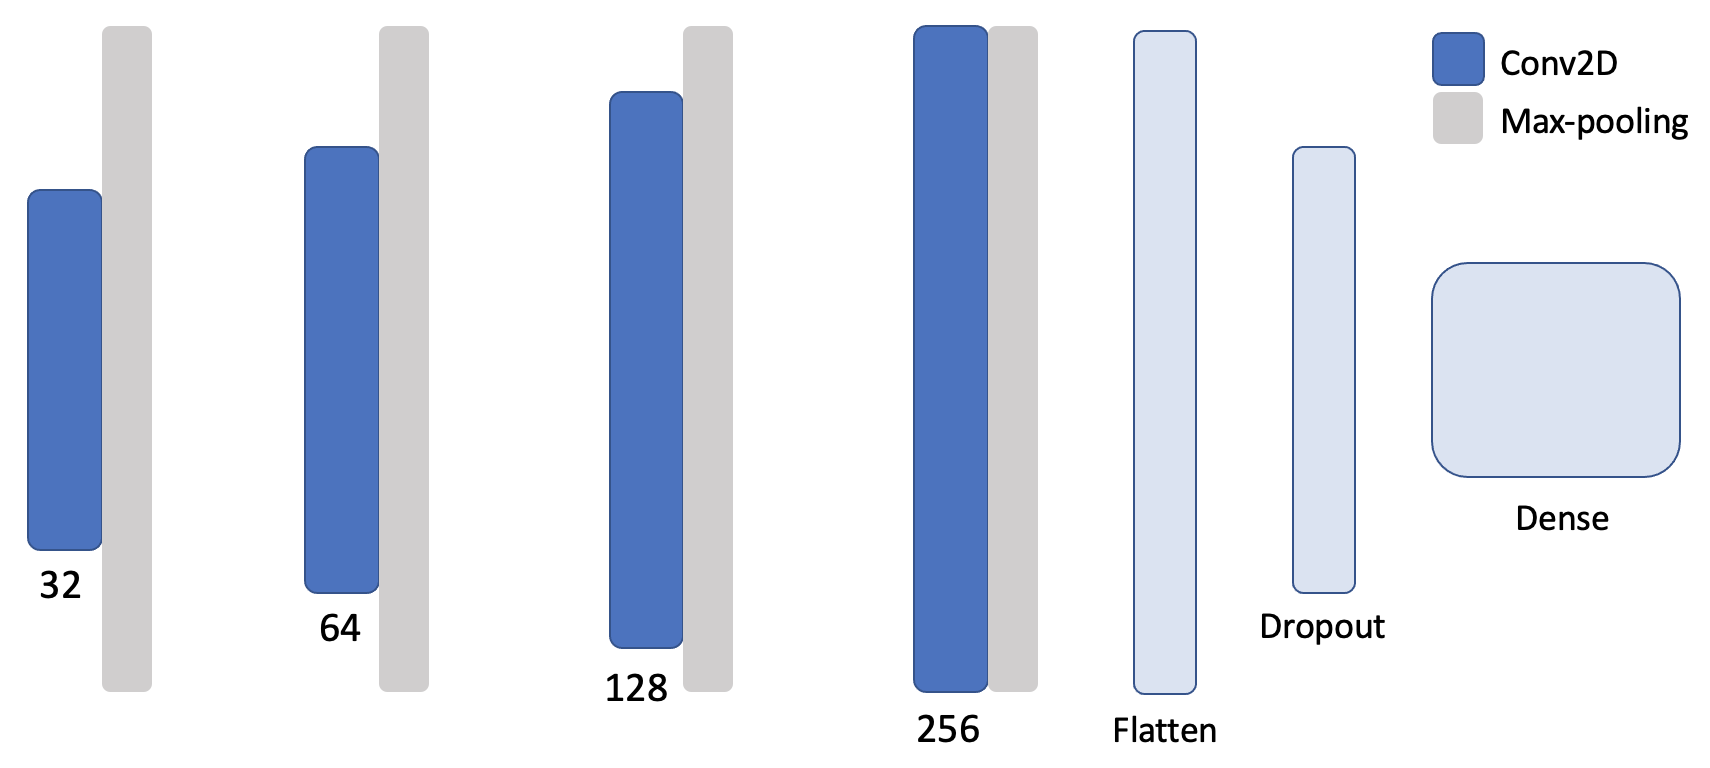
\includegraphics[width = \textwidth]{Figures/CNN_architecture.png}
    \caption{CNN representation with CNN-mc architecture on the top and CNN-hc architecture on the bottom\cite{SmallData}.}
    \label{fig:CNN_architecture}
\end{figure}

Results in \cite{SmallData} give evidence to support the use of CNN-hc when down-sampling but doesn't regard up-sampled or class weighted data. Given that up-sampling and class weighting will be the two methods implemented within this paper to deal with class imbalance, the table below gives a brief comparison of the different architectures on both up-sampled and class-weighted data for the binary classification task using mel-spectrograms. The results in Table~\ref{fig:compare_architectures} \todo{fix reference}show little variation between the average F1 score for the two architectures, apart from an increase for the minority class on up-sampled data. This alongside the results in \cite{SmallData} is reason to consistently use CNN-hc throughout this project.

\begin{table}[htbp]
\label{fig:compare_architectures}
\caption{F1 scores of two CNN architectures on up-sampled and class-weighted data.}
\begin{center}
\begin{tabular}{|c|c|c|c|c|}
\hline
\textbf{Country}&\multicolumn{2}{|c|}{\textbf{Up-sampled}}&\multicolumn{2}{|c|}{\textbf{Weighted}}\\
\cline{2-5}
\textbf{Pair} & mc & hc & mc & hc\\
\hline
\textbf{\textit{Usa/Spanish}} & 0.89/0.7 & 0.87/0.72 & 0.90/0.76 & 0.88/0.72
\\
\hline
\textbf{\textit{Usa/French}} & 0.94/0.47 & 0.92/0.4 & 0.92/0.33 & 0.93/0.52
\\
\hline
\textbf{\textit{Usa/German}} & 0.96/0.25 & 0.95/0.2 & 0.93/0.29 & 0.94/0.18
\\
\hline
\textbf{\textit{Spanish/French}} & 0.81/0.12 & 0.82/0.32 & 0.84/0.48 & 0.83/0.56
\\
\hline
\textbf{\textit{Spanish/German}} & 0.88/0.2 & 0.87/0.18 & 0.90/0.36 & 0.91/0.25
\\
\hline
\textbf{\textit{French/German}} & 0.73/0.2 & 0.76/0.36 & 0.74/0.46 & 0.74/0.46
\\
\hline
\textbf{\textit{Average}} & 0.868/0.323 & 0.865/0.363 & 0.872/0.447 & 0.872/0.448\\
\hline
\end{tabular}
\label{tab1}
\end{center}
\end{table}

\textbf{Data Balancing:} As is the case with most ASR systems today, our data is dominated by English native speakers(in our case American speakers). The difference between our smallest class(36) and largest(373) is considerable and therefore requires methods to better balance the data prior to training. Upsampling, downsampling and class weighting\todo{Possibly data augmentation????} will all been implemented in our project as a comparison for how best to approach the issue of data imbalance.

\begin{itemize}

\item Upsampling requires reproducing data in the smaller classes, increasing the size of the dataset to fit that of the largest class. It is particularly important here that the train test split is made prior to duplicating the data otherwise we could be testing on data that has already been trained on. \todo{mention that CNN learns more from larger class}

\item By downsampling the data we reduce the size of the larger classes to match that of the smallest class. This results in a balanced datasets however, given the size of our smallest class(36), the restriction could impede massively on the training process of the CNN.

\item Class weighting can be implemented with imbalanced data to direct the focus of the CNN on to the smaller classes. It forces the  prediction error to be greater for more heavily weighted classes. It is standard to set the weighting to be
\todo{Weighting has been corrected - Callum has put correct one in final.tex}
$$\frac{\text{size of largest class}}{\text{size of current class}},$$
relating the weights to the relative size of the classes.
\end{itemize}

In the case of up-sampling and weighting, the classes are still imbalanced in size so these methods will require an alternative metric to that of test accuracy for evaluation such as the F1 score.

\textbf{Regularisation:} Due to the lack of data available our model is even more inclined to over-fit. In an attempt to overcome this issue we have implemented numerous regularisation techniques.

\begin{itemize}
    \item As discussed in [https://arxiv.org/pdf/2003.12843.pdf] the CNN architectures we are implementing consist of a dropout layer. This regularisation technique randomly omits units from the neural network along with their connections to reduce co-adaptation between units[https://dl.acm.org/doi/pdf/10.5555/2627435.2670313]. [https://arxiv.org/pdf/2003.12843.pdf] gives evidence to support the use of dropout layers regardless of data scarcity, and produces best results using a dropout probability of $0.7$.
    
    \item Early stopping not only reduces overfitting but also computation time. By monitoring a chosen metric, the training process can be stopped under specified conditions before the model gets the chance to overfit the data. Optimising early stopping is highly dependent on the choice of metric and the patience; that is, the number of epochs with no improvement after which training will be stopped[$https://keras.io/api/callbacks/early_stopping/$]. It is common to use validation loss as the monitored metric \todo{find reference for this}. Further, the early stopping class in keras includes a parameter restore\_best\_weights which restores the weights of the epoch with the best monitored metric, in our case the validation loss. Given this parameter, we can set the patience to be reasonably high and still output the results of the epoch with the best validation loss. This will increase computation time but minimise the likelihood of both under- and over-fitting.
    
    \item Data Augmentation?(Mention breifly and)
\end{itemize}

%%%%%%%%%%%%%%%%%%%%%%%%%%%%%%%%%%%%%%%%%%%%%%
%% Results %%%%%%%%%%%%%%%%%%%%%%%%%%%%%%%%%%%%%
%%%%%%%%%%%%%%%%%%%%%%%%%%%%%%%%%%%%%%%%%%%%%%
\section{old lit review}

In recent years, accent detection has become a very prevalent area of study, heavily influenced by the increased use of ASR systems. Much of the work throughout this project has been developed from the many recent findings and, must therefore, be jointly accredited. Here, we will give a review of the literature that has been used to help build our approach.

Despite the fact that in speech recognition tasks one must initially deal with audio files, many researchers \cite{AudioSignals, SimpleSpeech, 7952132}[etc.] have found that converting audio files into different variations of images and running them through a CNN can have improved results. 

Converting audio files into images lends itself to the use of well-researched CNN architectures for image classification tasks such as AlexNet \cite{Alex_Net}, VGG Net \cite{VGG_Net} or ResNet \cite{Res_Net}. These approaches however, require a large dataset which we do not have access to. According to \cite{SmallData}, when implemented on a small dataset, low-complexity CNNs perform comparably well or better than state-of-the-art architectures. Additionally, \cite{SmallData, EnvSound} introduce the use of data augmentation for overcoming data scarcity, as well as the use of dropout layers for regularisation. For three different down-sampled datasets, the CNN architecture CNN-hc (32, 64, 128, 256 filters) \cite{SmallData}, with augmentation and a dropout layer with probability 0.7, outperforms all other architectures, including ResNet, when the sample size is less than or equal to 160 elements per class. Given that we are dealing with classes of similar order to those in \cite{SmallData}, the use of this architecture alongside data augmentation and a dropout layer would be a beneficial approach for our project.

The audio-to-image conversion is generally approached by coverting to either Mel Frequency Cepstral Coefficients (MFCCs) or Mel-spectrograms (Melgrams). All papers mentioned so far relating to audio classification \cite{EnvSound, 7952132, AudioSignals, SimpleSpeech} have used one of the two image variations. Both feature extraction methods use a mel-scale to adapt frequencies in the WAV files to be congruent with the natural auditory range of humans \cite{SimpleSpeech}. The scale emphasises high precision in the lower frequencies and low precision in the higher frequencies as is the case with the auditory system of humans\cite{MusicGenre}. One paper in particular \cite{SimpleSpeech} discusses clear comparisons between the two image types for neural network application. MFCC decorrelates features which, given that neural networks tend to perform well on correlated features, may impede on the performance of the CNN. For this reason it is more common to use melgrams, however we will apply both throughout this paper for comparison. 
\todo{Add more to this}
\section{Results}

\subsection{CNN}

Having processed the WAV files into both mel-spectrograms and MFCCs, the CNN model is executed and evaluated to distinguish the contrast of the two image variations and the effects of the different sampling methods that attempt to deal with data imbalance and data scarcity. 

A comparison of the two image variations is given in the table below.
\begin{table}[H]
\label{fig:}
\caption{Comparison of macro F1 scores for the two image variations on multi-class classification.}
\begin{center}
\begin{tabular}{|c|c|c|c|}
\hline
\multicolumn{2}{|c|}{\textbf{Mel}}&\multicolumn{2}{|c|}{\textbf{MFCC}}\\
\cline{1-4}
Upsampled & Weighted & Upsampled & Weighted\\
\hline
0.35 & 0.53 & 0.47 & 0.43\\
\hline
\end{tabular}
\label{tab1}
\end{center}
\end{table}

As expected from the various research papers[cite papers] there is clear improvement in macro F1 score, approximately $23\%$, when implementing the CNN using mel-spectrograms over MFCCs for the class weighted data. Notice however that this is not true for the upsampled data. This is likely a result of the limited window between underfitting and overfitting. Early on in the learning process the CNN begins to overfit the smaller classes due to the duplicated elements. As mel-spectrograms are more detailed images than MFCCs, less is learnt from the training process before being stopped due to overfitting. This is evident from the learning curves below.

\begin{figure}[H]
\begin{subfigure}[t]{0.237\textwidth}
  \centering
    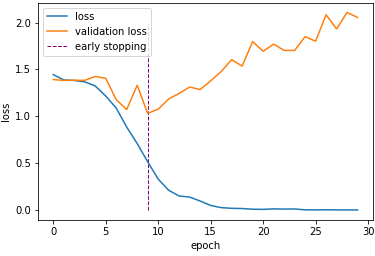
\includegraphics[width=\textwidth]{Figures/usa_spanish_french_german_mel_hc_upsampled_loss.png}
    \captionof{figure}{}
    \label{fig:}
\end{subfigure}
\hspace{0.005\textwidth}
\begin{subfigure}[t]{0.237\textwidth}
    \centering
    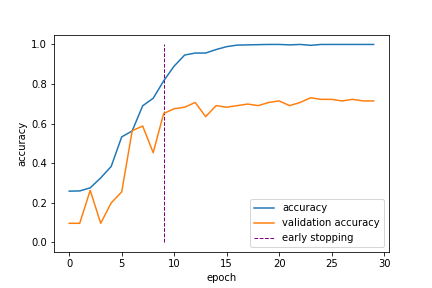
\includegraphics[width=\textwidth]{Figures/usa_spanish_french_german_mel_hc_upsampled_accuracy.png}
    \captionof{figure}{}
    \label{fig:}
\end{subfigure}
\caption{}
\label{fig:}
\end{figure}

The benefits of early stopping become apparent when observing the learning curves of the CNN model. Without the input from early stopping to reduce overfitting, the elements, especially those in minority classes, will likely be misclassified. The misclassification of minority classes opposes the pursuit for a model with improved identification of foreign accented speakers.

Results from the following tables of F1 scores\todo{reference} support the use of mel-spectrograms alongside class weighted data for the development of a non-biased accent identification system.

\begin{table}[H]
\begin{center}
\begin{tabular}{|c|c|c|c|c|c|}
\hline
\textbf{Image} & \textbf{Sampling}&\multicolumn{4}{|c|}{\textbf{Native Language}}\\
\cline{3-6}
\textbf{Type} & \textbf{Method}& Usa & Spanish & French & German\\
\hline
Mel & Upsampled & 0.71 & 0.58 & 0.12 & 0.00\\
\hline
Mel & Weighted & 0.80 & 0.47 & 0.67 & 0.18\\
\hline
MFCC & Upsampled & 0.82 & 0.71 & 0.35 & 0.00\\
\hline
MFCC & Weighted & 0.83 & 0.60 & 0.00 & 0.29\\
\hline
\end{tabular}
\label{tabl:}
\caption{Individual F1 scores for CNN.}
\end{center}
\end{table}




%%%%%%%%%%%%%%%%%%%%%%%%%%%%%%%%%%%%%%%%%%%%%%
%% Discussion %%%%%%%%%%%%%%%%%%%%%%%%%%%%%%%%%%%%%
%%%%%%%%%%%%%%%%%%%%%%%%%%%%%%%%%%%%%%%%%%%%%%

\section{Discussion}

%%%%%%%%%%%%%%%%%%%%%%%%%%%%%%%%%%%%%%%%%%%%%%
%% Conclusion %%%%%%%%%%%%%%%%%%%%%%%%%%%%%%%%%%%%%
%%%%%%%%%%%%%%%%%%%%%%%%%%%%%%%%%%%%%%%%%%%%%%

\section{Conclusion}

\begin{itemize}
    \item Mention this paper https://ieeexplore.ieee.org/stamp/stamp.jsp?tp=&arnumber=596139:
    
    Most information for accent detection is found in the 1500-2500Hz range compared to accent recognition which performs best on a mel-scale(higher precision for lower frequencies ). They back this up by showing an improved accuracy using an image variation for accent classification that focuses on this specific range compared to that of MFCC.
    
    \item Data Augmentation Improves Recognition of Foreign Accented Speech
    https://www.isca-speech.org/archive/pdfs/interspeech_2018/fukuda18_interspeech.pdf
    
    Comparison of different data augmentation methods for foreign accented speech recognition. Most improvements using speed pertubation, speeding up or slower down speech in Wav files.
\end{itemize}


\printbibliography

Possible book to look into:
https://ieeexplore.ieee.org/book/5263814

\newpage

\end{document}